\section{Framework}
\label{sec:framework_short_desc}
This project involves processing a large amount of data, requires a lot of computational power and working as a team with heterogeneous environments. Since we had anticipated the need to make a lot of experiments, we carefully designed a framework which allows training and to keep a record of all experiments while having a reproducible code. All explanations on the framework we developed have been listed in appendix \ref{sec:training_fwk} . As a matter of fact, getting an accurate system for this task was also a software engineering challenge and not only a pure machine learning task. Our code is available on ~\href{https://github.com/balthazarneveu/molecule-retrieval-using-nlp}{GitHub} for future work.

\section{Our work}

\subsection*{Base model}
Figure \ref{fig:original_pipeline} depicts our approach to this task: Text descriptions are transformed into sequences of tokens of various lengths (sequences of integers). Tokenized sequences are then embedded into a vector space using a large language model encoder. Throughout the project, we used \textbf{various versions of the BERT}\cite{bert} architecture (which is the encoder part of the Transformer \cite{transformer} which have been pretrained with a masked language modeling task). Each description $T_{i}$ is transformed into a vector $t_{i}$ (text descriptions embeddings) by extracting the representation of the \textbf{first token} (the CLS token).

Molecules $M_{i}$ will be transformed into vector descriptors $m_{i}$ (molecule embeddings). Each molecular structure (more generic than an atom) is first transformed into a vector using Mol-2-Vec \cite{mol2vec} which incorporates a lot of prior knowledge about chemistry into each node vector. The whole molecule structure is kept as an undirected graph to model the bounds between elementary molecular structures. \textbf{A graph convolutional network (GCN)} is then used to embed these graphs into a vector space. The molecule and text descriptions embeddings are then compared.

\textit{Contrastive learning is used to train such a model}: supervision comes from the knowledge of the pairing between the molecule and its text description. We compute a pairwise similarity between the molecule embedding $m_{j}$ and text embeddings $t_{i}$ and maximize it when $i=j$. 
% The idea behind contrastive learning relies on maximizing similarity between molecules and text embeddings for the correct pair and minimized for the wrong pairs.

\textit{Categorical cross entropy for contrastive learning}: The loss we're using for the baseline is $L(m, t) = \text{CCE}(m^{T}.t , \mathbb{I}_{b} )+\text{CCE}(t. m^T , \mathbb{I}_{b})$. where $t, m \in \mathbb{R}^{d, b}$ with embedding dimension $d=768$ are respective batches of text and molecule embeddings of size $b=32$.

$\text{CCE}(m^{T}.t , \mathbb{I}_{b}) = \sum_{i=1}^{b} l_{i}$ 

with $l_{i} =-\text{ln}(\text{softmax}(m^{T}.t_{i})) = -\text{ln}\frac{e^{m_{i}^T.t_{i}}}{\sum_{j=1}^{b}e^{m_{j}^T.t_{i}}}$


% \textit{At inference time}, a chemist will query the system with a text sentence $T$ to search the database. The sentence query will be embedded into a vector $t$ which is compared to all molecules embeddings in a database. The most relevant molecules (highest similarity score) can be proposed to the chemist.

\subsection*{Preliminary study (baselines)}
\label{sec:preliminary study}

\begin{table*}[h]
    \centering
    \begin{tabular}{|c|c|c|c|c|}
    \hline
    \textbf{Experiment ID} & \textbf{Model Size} & \textbf{LLM} & \textbf{GNN} & \textbf{LRAP} \\ \hline
    101         & 593k                & Frozen Distill-Bert           & Base 3 layer GCN       & 18.7\%      \\ \hline
    106         & 964k                & Frozen Distill-Bert + Adapter & Base 3 layer GCN       & 26.8\%      \\ \hline
    114         & 2.125M              & Frozen Distill-Bert + Adapter & Big 5 layer GCN        & 31.6\%      \\ \hline
    112         & 964k                & Frozen Sci-Bert + Adapter     & Base 3 layer GCN       & 36.7\%      \\ \hline
    113         & 2.125M              & Frozen Sci-Bert + Adapter     & Big 5 layer GCN        & 39.8\%      \\ \hline
    65          & 66.9M               & Trainable Bert                & Base 3 layer GCN       & 63.5\%      \\ \hline
    400         & 110M                & Trainable Sci-Bert            & Base 3 layer GCN       & 66\%        \\ \hline
    \end{tabular}
    \caption{Base models specifications and performances - Trained with batches of size 32 using the Adam optimizer \cite{adamKingma} (Learning Rate $=10^{-4}$ Weight decay $10^{-2}$) to minimize the Categorical Cross Entropy loss applied to contrastive learning.}
    \label{tab:preliminary_study_metrics}
\end{table*}


We begin with a few toy experiments to see which architecture factors are most promising (initial hope is that the performances will scale accordingly when we add all extra machine learning tricks).

\textbf{Frozen LLM weights}: We started with simple models based on the base GCN (3 graph convolution layers followed by a global pooling layer and 2 layers MLP). Instead of fine tuning all parameters of the LLM, we first froze the LLM parameters. Although simple, this idea intuitively has many advantages for training:
\begin{itemize}
    \item We discard the huge memory cost of training a LLM (memory issues not only come from storing the weights on the GPU but from all the optimizers variables during back propagation). \textit{The idea could have been pushed further by pre-computing the text embeddings and storing them on disk.}
    \item Intuitively, freezing the LLM parameters should make the training more stable as the LLM embeddings acts as a kind of anchor that the GNN shall match.
\end{itemize}
Unfortunately, training achieves a low LRAP score (\textit{not too surprisingly since the number of parameters to train is relatively low}). We added an "adapter" module which is simply a MLP which project the text representations into a more adapted space which can be matched with the graph embeddings.

\textbf{Influence of the graph neural network size}: We pursued our explorations to see the impact of the GNN size. The \textbf{big GCN} (5 graph convolution layers with 2 residual connection) is more complex and has more parameters to train. We can see that the LRAP is improved by increasing the GCN size. 
\begin{itemize}
    \item Using frozen Distil-BERT: from experiment 106 (base GCN $\text{LRAP}=26.8\%$) to 114 - (big GCN $\text{LRAP}=31.6\%$)
    \item Using frozen SciBERT: from experiment 102 (base GCN $\text{LRAP}=36.7\%$) to 113 - (big GCN $\text{LRAP}=39.8\%$)
\end{itemize}


\textbf{Influence of the pretrained language model}: We also browsed Hugging Face to find models that could be dedicated to scientific-specific language processing. Sci-Bert\cite{scibert} (used in Text-2-Mol\cite{text2mol}) can be used as a drop-in replacement for the Distil-Bert baseline model. Improvements were two-fold when changing the pretrained LLM during this preliminary study: a tokenizer dedicated to a scientific corpus (SciVocab) seems by nature a natural choice for scientific words... (\textit{molecule names not being too frequent in common language}). The Sci-Bert model may also have reasoning capabilities closer to science and chemistry reactions as it's been trained on one million scientific papers (a total of over 3 billions of tokens, similar to BERT). This was translated by a improvement in performances. Increasing the GNN size improves accuracy.

\begin{itemize}
    \item Using the Base GCN : from experiment 106 Distil-BERT ($\text{LRAP}=26.8\%$) to experiment 112 - SciBert ($\text{LRAP}=36.7\%$).
    \item Using the Big-GCN: from experiment 114 Distil-BERT ($\text{LRAP}=31.6\%$) to experiment 113 - SciBert ($\text{LRAP}=39.8\%$).
\end{itemize}
The capacity of the network (same number of parameters) being fixed between these two experiments, it proves that the SciBERT pretraining with SciVocab tokenization is definitely more suited for our task. We hoped that this $> 8\%$ LRAP improvement would be translated when training a fully trainable LLM.

Unfortunately we later conducted larger experiments with fully trainable LLM (starting from the pretrained weights) and the performances improvements due to the previous modifications did not fully apply. Using the Base GCN : from experiment 65 Distil-BERT ($\text{LRAP}=63.5\%$) to experiment 400 - SciBert ($\text{LRAP}=66\%$), there's not that $seq 8\%$ LRAP improvement that we had seen earlier. Furthermore, it's hard to tell whether the 2.5\% improvement is due to the SciBert model pretraining being more suited for our task or the fact that the model has nearly twice as many trainable parameters than the Distil-BERT model. 

This preliminary study gave us guidance that using a larger GCN and using SciBERT pretrained weights and tokenizer were good trends to follow to try improving our results. The pitfall is that fine tuning SciBERT comes with a bigger memory footprint than Distil-BERT which requires diminishing batch sizes for a fixed GPU (large batch size seems to be one key factor of the success of contrastive learning when looking at CLIP \cite{CLIP}). Experiments 65 and 400 have been cautiously trained with \textit{the same batch size of 32} and same hyperparameters to get comparable results: 
\begin{itemize}
    \item the SciBERT experiment 400 could only be ran using a NVIDIA RTX A4000 with 24Gb of RAM
    \item the Distil-BERT experiment 65 was possible on a NVIDIA Tesla T100 with 16Gb of RAM (Kaggle Kernels notebook).
\end{itemize}



\begin{figure}[ht]
    \centering
    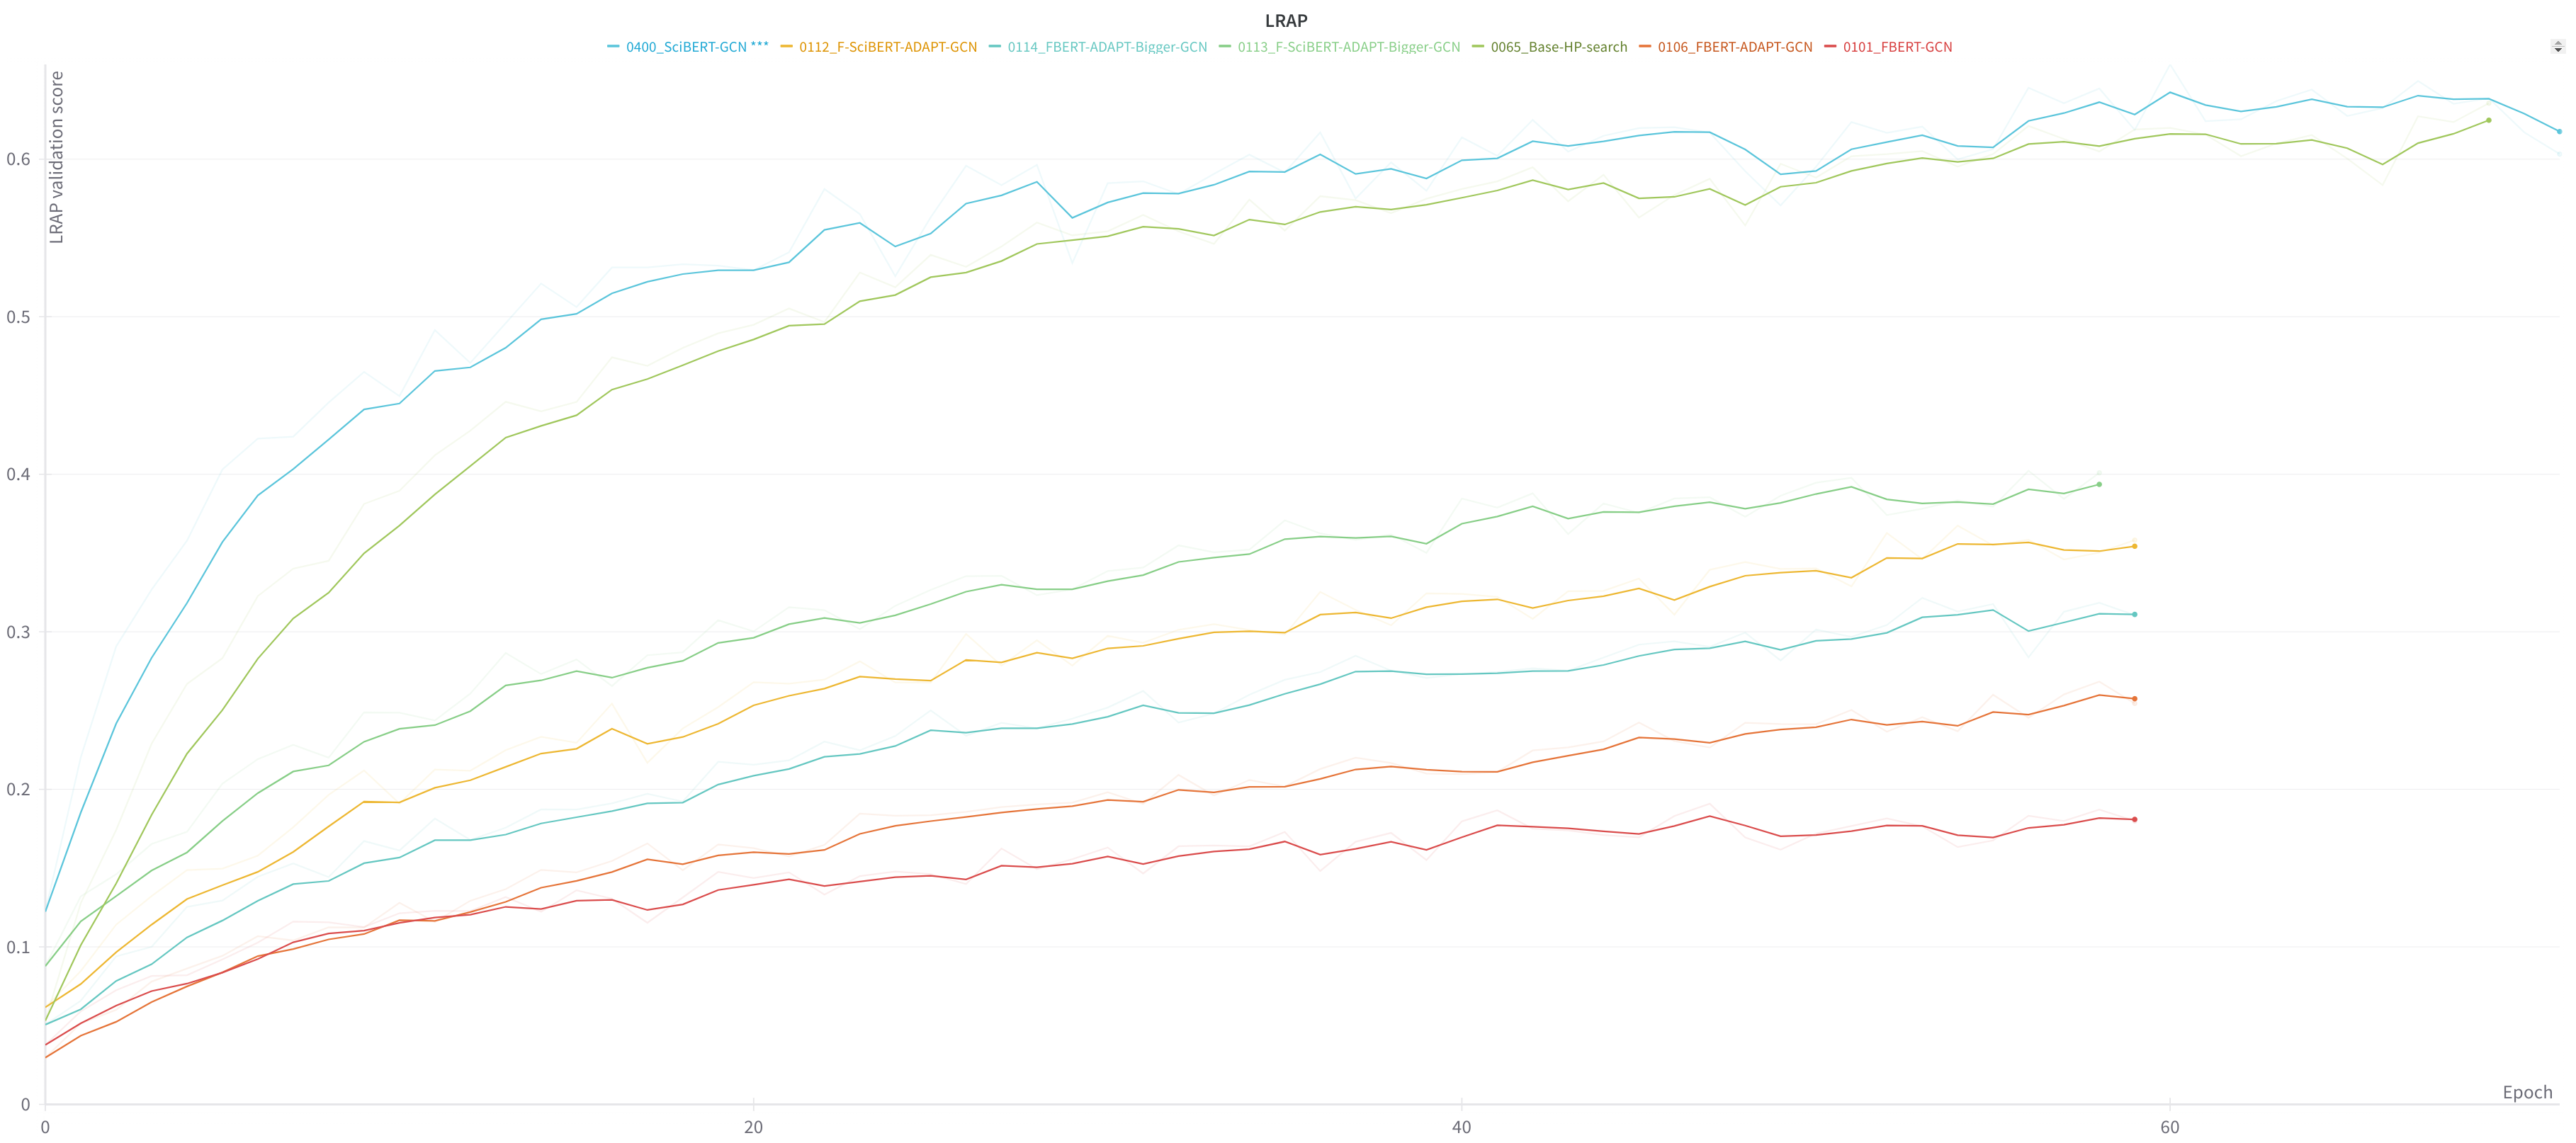
\includegraphics[width=0.5\textwidth]{figures/preliminary_study.png}
    \caption{Training curves for the preliminary study.}
    \label{fig:preliminary_study_curves}
\end{figure}


\subsection*{Our model}
\label{sec:our model}
We have trained and experimented with several models throughout this project. We identified axes which left room for improvement of the LRAP score and we tried to combine them to create the most robust and efficient model. 

\subsubsection*{Research on the LR parameter}
\hfill\\
When running tests on the baseline with different hyperparameters, it became obvious that the model was very sensitive to the learning rate. We empirically identified an ideal learning rate parameter to train our best experiment on the baseline. In experiment 68 we trained the baseline model with this optimal learning rate of $lr=7e-5$ and a batch size of 128 and achieved 68\% of accuracy. 
\newline We also implemented a learning rate scheduler. We tried cosine annealing which did not prove very efficient and ended up working with a plateau learning rate scheduler for most of the following experiments.

\subsubsection*{LoRa}
\hfill\\
Because of the nature of the LRAP metric, a key element to improve the LRAP was to be able to increase the batch size, which was hard to do here given the nature of the data. We implemented LoRa to reduce the number of parameters which need to be trained for the LLM (only 1\% left approximately) and to be able to increase the batch size during training. 
\\ This technique however did not prove as efficient as expected. It led to no major improvement on the batch size when using Scibert (we were not able to go beyond batches of size 64). When adding Lora to the baseline model and using Scibert (experiment 502) with a batch size of 64 (the biggest we could fit on the GPU) and a learning rate of $3.10^{-4}$, we only obtained a 60\% LRAP score, which was not an improvement over the best baseline model mentioned in the previous subsection. The same baseline model with DistilBert  and batch size 128 (experiment 514) achieved a LRAP score of 68\% matching the previous model. This also showed that using SciBert was not necessarily helping achieve better accuracy but rather adding constraints to our trainings regarding batch sizes.
\newline
Using LoRa proved more efficient when using DistilBert, where it enabled us to train experiments with bigger batches. Experiments 577 and 9011 have the same architecture (5 layer GCN, learning scheduler with the same parameters, DistilBert) except for the fact that 577 uses LoRa and trains batches of size 192 and 9011 trains simply batches of size 180 without LoRA. In the end, we noticed a gap in performance since 9011 scored a LRAP of 86\% while 577 only scored 74\%, the bigger batch size did not make up for the performance decrease caused by the reduction of trainable parameters of the LLM. 
\newline
This led us to use LoRA when experimenting on other axes such as the influence of the GCN architecture or the learning rate scheduler and take advantage of the increased speed of the training, but to drop it for experiments with a high LRAP score potential. However, in some situations which we cannot fully explain we still obtained good results when training with Lora and Scibert with architectures such as that of experiment 573 which achieved 80\% in LRAP score and which we reused later.
(See Appendix \ref{sec:lora} for detailed information on the experiments)

\subsubsection*{GCN}
\hfill\\
As previously mentioned, we had identified the GCN as a promising work direction to improve the accuracy of our model. After testing the difference with a Frozen LLM, we compared the different GCN architectures when using SciBert and LoRa for the LLM. This confirmed our intuitions, namely that accuracy improves when we increase the size of the GCN for otherwise similar models. The results and architectures of these experiments can be found in Appendix \ref{sec:gcn} The gap in performance can however be reduced when increasing the size of the batches during the training for models with a smaller GCN architecture.
\newline
After this round of experiment, we stopped working with Scibert and used only DistilBert. We ran several very successful experiments by toying with hyperparameters such as the batch size and the architecture of the GCN. The models, architectures and scores are detailed in Appendix \ref{sec:best_old}. 
We noticed that we could make up for the lack of performance of the "bigger GCN" compared to the "Fat GCN" by increasing the batch size. The "Fat GCN" was also slower in training and could not be scaled as easily. 
The results of these four experiments were all used for our final model and included in the ensembling.

\subsubsection*{Loss functions for the training}
\hfill \\
All previous experiments were trained using the contrastive loss .
Following the idea of Text-2-Mol \cite{text2mol}, we changed the training loss. We replaced the categorical cross-entropy loss by one derived from the binary cross entropy. In doing so, we consider that our problem is no longer a multi-class problem (one label per pair of molecule and description) but rather a binary classification problem. This loss will be refered to as the 'binary contrastive loss' both in this report and our code. 
We repeated the baseline experiments with this new loss with different batch sizes in experiments 18, 19 and 20 which are detailed in Appendix \ref{sec:baseline_new}. We noticed a big improvement over the 66\% we had achieved on the baseline when training on the contrastive loss. We also observed that the trainings were even more sensitive to the learning rate parameter and the performance did not scale as well as hoped when increasing the batch size. 
\newline
We reproduced variants of the experiments 9008 to 9011 which had yielded high scores when trained with the contrastive loss. Again, by playing with the GCN architecture, the batch sizes and adding a learning rate scheduler, we were able to launch some effective experiments.  After 200 epochs, our most successful experiments 9075 and 9077 had an LRAP score of over 86\% on the valid set, and were trained with a smaller batch size than 9008-9011. Their descriptions and scores are visible in Appendix \ref{sec:best_new}.
We included the outputs of 9075 and 9077 in the ensembling which was used to elaborate our final best model.

\subsubsection*{Freezing the LLM, training a large GCN from scratch} \hfill\\
We have finally experimented with an improved version of the idea we had at the beginning of freezing the weights. We reused models we had previously train jointly which had yielded correct LRAP scores. We assume that the LLM is able to create rich text features which are relevant to our molecule corpus. We froze the weights of the pre-trained model in order to reduce the GPU memory used during training. We are now able to train a larger GCN from scratch (or fine tune our pre-existing one with bigger batch sizes, see table ~\ref{table:ft_gcn_model_memory_occupancy}). This idea allowed us to start from a language model pretrained using SciBERT (and FatGCN) using batches of size 64 (trained on a Nvidia A5000) which was stuck at a LRAP score of 0.8 (experiment 753). We trained a new GCN from scratch using batches of size 256 leading to 0.87 LRAP score (trained on a much smaller GPU RTX 2090)(see Appendix \ref{sec:frozen} for more information)

\begin{table}[!]
    \centering
    \begin{tabular}{|cccc|}
    \hline
    % \textbf{LLM} & \textbf{Batch Size} &\textbf{GPU Utilization}& \textbf{GPU Memory Occupancy} \\ \hline
    \textbf{LLM} & \textbf{Batch Size} &\textbf{GPU Utilization}& \textbf{GPU Memory} \\ \hline
    Trainable & 8 & 90\% & 2.95 GB \\
    Frozen & 8 & 91\% & 0.913 GB \\
    Frozen & 32 & 100\% & 1.29 GB \\
    Frozen & 128 & 100\% & 2.97 GB \\
    \hline
    \end{tabular}
    \caption{Comparison of memory occupancy for different model configurations on NVIDIA T500 with 4GB of GPU Memory. GCN Model is the FatGCN. LLM is a SciBERT model that we trained from scratch with LORA. This allows putting much larger batch sizes in the GCN model (from batches of size 8 when training LLM and GCN jointly to 128 - please note that the trainable LLM memory in the first row is already reduced a lot by using LoRA compared to traing all parameters at once).}
    \label{table:ft_gcn_model_memory_occupancy}
\end{table}
\subsubsection{Final Model}
In the end, after having extensively experimented with different architectures by changing the GCN, the LLM, the batch size and the learning rate, we obtained seven different models with acceptable LRAP scores: 9008, 9009, 9010, 9011, 9075, 9077 and 611.
We applied an ensembling technique to average the scores of each of these models which leads to an extra LRAP score improvement as suggested in \cite{text2mol}. (average submission csv for experiments 9008, 9009, 9010, 9011, 9075, 9077 and 611 basically, a trick which has no extra cost and allows taking more confident decisions). Our final model averages the outputs of seven different models which each take 12 to 13 hours: 91 hours of computation were hence required to obtain this model.
The best LRAP score of any single one of these models was around 86.5\% and we managed to reach a score above 90\% thanks to this technique.
